% Unofficial Chinese translation of the exact arXiv:2509.14234v3 version.
% Dependencies in integrating main: authorized fixed template, graphicx, booktabs, longtable, fvextra.
\originalchapter{计算即教师：将推理计算转为无参考监督}\label{cat-paper}
原作：Dulhan Jayalath\textsuperscript{1,\dag}、Shashwat Goel\textsuperscript{2,3,\dag}、Thomas Foster\textsuperscript{1,5}、Parag Jain\textsuperscript{5}；\par
\noindent Suchin Gururangan\textsuperscript{4,\dag}、Cheng Zhang\textsuperscript{5}、Anirudh Goyal\textsuperscript{5}、Alan Schelten\textsuperscript{5}.
单位：\textsuperscript{1}牛津大学；\textsuperscript{2}ELLIS Institute Tübingen；\textsuperscript{3}马克斯·普朗克智能系统研究所；\textsuperscript{4}Anthropic；\textsuperscript{5}Meta Superintelligence Labs. \textsuperscript{\dag}表示该工作在 Meta Superintelligence Labs 完成.
通信地址：\texttt{dulhan@robots.ox.ac.uk}、\texttt{agi@meta.com}、\texttt{alanschelten@meta.com}.

指定原文为 \url{https://arxiv.org/abs/2509.14234v3}，v3 日期 2026 年 5 月 9 日，首次提交日期 2025 年 9 月 17 日. 指定 PDF 首页面内日期为 2026 年 5 月 12 日，而同版本 HTML 的内部日期显示 2026 年 8 月 24 日；源文件使用排版时日期宏，二者均与固定的 arXiv 版本日期分开记录. 该版本官方页面的许可证链接指向 CC BY 4.0：\url{https://creativecommons.org/licenses/by/4.0/}. 本译稿由 ai-self-study contributors 以机器辅助方式译制，非官方译本. 改动包括完整中文翻译、授权固定版式重排、交叉引用与图表编号适配、术语表及单独标记的译者说明. 原书目元数据、模型与程序标识符、XML 标签和必要输出标记保留原文. 论文原图或由原作者 TikZ 代码导出的矢量图逐图署名，图内英文标注保留. 未复制原稿的公司标志、文档类或字体文件. 会议版本仅用于版本信息对照，本文翻译和许可依据不与它混用. 下文“我们”均指原作者.

\begin{remark}
译者说明：伪参考是由模型生成的监督估计，不等于外部真值. 二元评分细则由模型提议并由模型判别，仍可能有遗漏、错误和共同偏差. 数学领域的答案匹配奖励只检验与伪参考的一致性；医疗领域的实验分数也不能直接当作临床真实性或安全性的证明. 以下正文忠实保留原作的结论和数值，这些说明与正文分开.
\end{remark}
\originalsection{摘要}\label{cat-abstract}
后训练没有真值时，学习信号来自哪里？我们表明，推理计算本身可以充当监督. 通过生成并行采样轨迹并将它们转化为参考估计，模型可以不依赖人类标签而学习；关键是，这甚至适用于医疗指导等不存在程序化检查器的不可验证领域. 我们把框架称为“计算即教师”（Compute as Teacher，CaT），它把并行采样轨迹的推理时计算转化为 RL 训练监督. 框架有两个组件：参考估计把轨迹聚合成伪参考答案，奖励推导把伪参考转化为 RL 奖励. 对前者，我们探索一种称为合成的简单方法，但框架接受任意聚合器；对后者，我们为不可验证领域提出自提出评分细则，即从伪参考生成、由大语言模型判别器计分的二元、可审计标准. HealthBench 上，CaT 训练模型达到或超过推理时聚合质量，而测试时计算减少 9 倍. 在这里，CaT 也可与使用专家医师标注的学习方式竞争，相对初始策略最高改善约 30\%. 框架自然扩展到可验证奖励，在 MATH-500 的测试时 RL 设置下达到最佳已有基线表现，展示跨两类领域的即插即用能力.

\originalsection{1 引言}\paperlabel{1}{cat-sec:introduction}
为获得专门技能而后训练大语言模型，通常依赖带标签参考答案的监督微调\cite{cat-long2022training,cat-wei2022finetuned}，或依赖程序化检查器提供可验证奖励的强化学习. 这种检查器只适用于数学、代码等形式正确性可计算的狭窄领域\cite{cat-lambert2024tulu,cat-shao2024deepseekmath}. 同时，许多有价值任务也没有标注参考答案. 在答案具有定性性质的不可验证场景中，如临床或生活方式指导\cite{cat-arora2025healthbench}、自由对话\cite{cat-roller2020open}和创意写作\cite{cat-paech2023eq}，可能存在多个有效答案，专家可能意见不同，确定性规则检查难以实施. 因而实践者常退回难以扩展的标注流程，或仅靠判别器反馈：让另一大语言模型为自由输出给粗粒度分数，尽管这种方式存在不一致、偏好冗长回答和奖励投机等已知问题.

\begin{figure}[ht]
\centering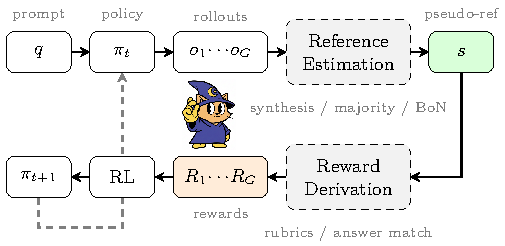
\includegraphics[width=.94\textwidth]{../papers/translations/cat/figures/framework.pdf}
\caption{CaT 框架. 策略 $\pi_t$ 为提示 $q$ 生成 $G$ 条轨迹. 参考估计通过合成、多数投票或 best-of-N，将它们聚合为伪参考 $s$. 奖励推导依据 $s$ 为每条轨迹计分：可验证领域使用答案匹配，不可验证领域使用自提出评分细则. 奖励驱动 RL，更新策略. 原图：Dulhan Jayalath 等，完整作者名单见文首，CC BY 4.0；由原作者 TikZ 导出，英文标注保留.}\label{cat-fig:framework}
\end{figure}
本文转而提出一个简单问题：\emph{推理计算能否替代缺失的监督？}

\textbf{计算即教师.} 我们回答“能”. CaT 用参考估计和奖励推导两个组件，把推理计算转成监督. 关键是，并行轨迹对模型的不确定性进行采样，因为它们恰好在模型不确定之处分歧. 一条轨迹可能有正确中间步骤，另一条有正确最终答案，第三条有有用验证；总体集合比单条包含更多信息. 参考估计把分散信息聚合为一个伪参考，奖励推导依据它为轨迹计分，以用于 RL. 框架不依赖具体聚合方法：多数投票、best-of-N 等选择策略找回最佳轨迹，生成策略则组合各轨迹片段，构建新回答. 我们探索简单的合成策略，让冻结策略条件于轨迹集合构建新回答，但任意聚合器都可接入同一奖励推导机制. GRPO 等组式 RL 已经为优势估计生成并行轨迹，因此参考估计增加的开销很小.

\textbf{不可验证领域的无参考奖励.} 奖励推导因领域而异. 数学、代码等可验证场景中，简单检查轨迹答案是否与伪参考一致. 更难的是没有这种检查的不可验证领域. 我们提出另一项关键贡献——自提出评分细则，让模型生成刻画伪参考的二元标准，如“建议咨询医疗专业人员”“指出患者对心律失常的担忧”. 独立大语言模型判别器逐项检查，奖励为满足标准的比例. 由此，不依赖真值也能为每条轨迹给奖励，在不可验证领域进行无参考 RL.

\textbf{有效原因的直观解释.} 轨迹从模型不确定性采样，分歧揭示了模型犹疑之处. 合成迫使模型检查分歧，依据证据选择一个观点或构建调和方案；选择方法只能挑一个已有答案. 不可验证领域的细则问“回答是否满足标准 X”，而非“回答好不好”；分解把模糊判断变成细粒度二元检查的求和，使验证更容易. 关键是，从伪参考自提出细则后，CaT 无需任何人类标注参考答案，就能为不可验证领域的轨迹提供奖励.

\textbf{实用性.} 框架实用且即插即用，无需人类标签、领域专用验证器，并复用标准 RL 已花费的组采样计算. CaT 把推理时聚合的收益摊入模型权重，在达到或超过聚合表现的同时，把每次查询的测试时计算最多减少 9 倍. 训练后策略回答质量还常超过初始聚合伪参考，并持续改进，直到轨迹趋于相似回答. 我们在 Gemma 3 4B、Qwen 3 4B、Llama 3.1 8B 三个模型家族，以及不可验证 HealthBench 和可验证 MATH-500 上验证.

\textbf{CaT 连接多条研究路线.} 它像自训练\cite{cat-schmidhuber2003exploring,cat-schmidhuber2013powerplay,cat-silver2016mastering,cat-silver2018general}和知识蒸馏\cite{cat-hinton2015distilling}一样，从模型生成监督学习，但通过调和多个样本产生目标，而非信任单个自标签. 它像多数投票、best-of-N 等测试时扩展方法一样利用并行轨迹，但通过 RL 把改善摊入权重. 相比大语言模型充当判别器的奖励\cite{cat-zheng2023judging}，细则评分提供分解、具体的标准，缓解不稳定和偏见\cite{cat-dineen2025qa,cat-gunjal2025rubrics}. 最后，CaT 把学习扩展到没有形式检查器的领域，补充程序化验证\cite{cat-lambert2024tulu}.

\textbf{贡献：}
\begin{enumerate}
\item 不可验证 RL 的自提出评分细则：将判断分解为二元标准的奖励机制，让没有程序化检查器的领域也能进行无参考 RL.
\item 计算即教师：通过参考估计和奖励推导，把推理计算转成监督的一般范式，合成是其中一种有效参考估计器.
\item 全面经验研究：三个模型在 HealthBench 与 MATH-500 上取得增益，训练模型用少 9 倍计算达到或超过推理时质量.
\end{enumerate}
\textbf{文章安排.} 第\ref{cat-sec:relatedwork}节讨论相关工作；第\ref{cat-sec:method}节形式化框架和自提出细则；第\ref{cat-sec:experiments}节给出实验设置；第\ref{cat-subsec:main-results}节给出结果、消融与分析；第\ref{cat-sec:discussion}节讨论局限、未来方向并总结.

\originalsection{2 相关工作}\paperlabel{2}{cat-sec:relatedwork}
\textbf{无参考微调.} 自生成监督在大语言模型训练中历史悠久. Constitutional AI\cite{cat-bai2022constitutional}用自我修订的生成结果训练，Self-Instruct\cite{cat-wang2023selfinstruct}生成并筛选自身的指令遵循数据，Quiet-STaR\cite{cat-zelikman2024quiet}在没有参考轨迹时学习产生推理 token. 它们针对无害性、指令遵循和推理等专门能力. CaT 更一般：只要模型能生成多样轨迹，且不可验证领域中的细则判断可靠，就支持无人工参考的 RL.

\textbf{无参考 RL.} 近期工作探索无真值标签的 RL. TTRL\cite{cat-zuo2025ttrl}用多数投票共识作数学伪标签，Absolute Zero\cite{cat-zhao2025absolute}在自行提出的数学和代码问题上自博弈. 这些方法有效，但局限于正确性可由程序检查的领域. 另一条路线最小化熵或最大化自确定性\cite{cat-zhao2025learning,cat-agarwal2025unreasonable,cat-prabhudesai2025maximizing,cat-gao2025one,cat-li2025confidence}. Wen 等\cite{cat-wen2025unsupervised}依据互可预测性为多项选择答案评分. 这些方法具有判别性质，只选择或评分已有输出. CaT 可用任一方法作参考估计器，也能超越选择；如果采用合成，它可构建采样集合分布之外的伪参考. 更重要的是，CaT 通过自提出细则扩展到不可验证领域，先前方法尚未用于这种设置；我们将其改为基线时，表现不及 CaT（第\ref{cat-subsec:ref-estimation}节）.

\textbf{测试时扩展.} 并行轨迹长期用于改善推理表现. 多数投票或自一致性\cite{cat-wang2023}选最常见答案；best-of-N 依信心、困惑度或大语言模型判断选择\cite{cat-zheng2023judging}. 它们提升准确率，却不把收益写入权重，每次部署都承担完整 $G$ 条轨迹成本. CaT 用同样轨迹生成 RL 监督，把推理计算摊入训练. 训练后模型以 $1/G$ 测试时成本达到或超过聚合质量，因此大部分计算在训练中一次性花费，而非推理时反复支付.

\textbf{不可验证 RL.} 无法程序化验证时如何产生奖励？已有方法假定可访问参考答案. VeriFree\cite{cat-zhou2025reinforcing}、JEPO\cite{cat-tang2025beyond}和 RLPR\cite{cat-yu2025rlpr}计算参考答案在模型推理链条件下的概率. Rubrics as Rewards（RaR）\cite{cat-gunjal2025rubrics}从参考答案构建评价细则，再由大语言模型判断评分，展示细则奖励优于直接评分. 我们继承此认识，但完全消除参考依赖：CaT 从轨迹估计的伪参考自提出细则. 推理计算生成伪参考，伪参考生成细则，细则生成奖励；流程没有人类标注进入.

\originalsection{3 计算即教师}\paperlabel{3}{cat-sec:method}
CaT 通过参考估计和奖励推导两个组件将推理计算转为监督，图\ref{cat-fig:framework}展示框架. 给定提示 $q$，当前策略 $\pi_t$ 生成 $G$ 条并行轨迹 $o_{1:G}$. 它们在模型不确定之处不同，因而采样其不确定性. 参考估计聚合为单个伪参考回答 $s$，用作监督目标. 奖励推导依据 $s$ 为每条 $o_i$ 产生 RL 奖励 $R(o_i;s)$.

框架不依赖具体聚合方法. 多数投票和 best-of-N 从已有轨迹选一个 $s$；合成等生成策略条件于全部轨迹构建新的 $s$，可能组合分散在集合中的正确片段. 本文经验探索合成，但奖励推导机制，尤其不可验证领域的自提出细则，可以配合任意参考估计策略.

\textbf{记号.} $q$ 为提示，$o_i$ 为采样轨迹，$s$ 为伪参考，$\mathcal R=\{r_j\}$ 为由二元标准组成的细则，$\pi_t$ 为第 $t$ 步当前策略，$\pi_0$ 为冻结锚点即初始策略，$\pi_J$ 为细则计分的判别模型.

\subsection*{3.1 参考估计}\paperlabel{3.1}{cat-subsec:ref-estimation}
参考估计把 $G$ 条轨迹聚合成一个伪参考 $s$，任意聚合策略均兼容，包括：
\begin{itemize}
\item 多数投票：$s$ 为 $o_{1:G}$ 中最常见的最终答案\cite{cat-zuo2025ttrl}，只适用于可比较答案的可验证领域.
\item Best-of-N：对某评分函数 $f$，令 $s=\arg\max_{o_i}f(o_i)$；可使用模型困惑度\cite{cat-agarwal2025unreasonable}、信心启发式\cite{cat-li2025confidence}或判别器分数.
\item 合成：冻结锚点 $\pi_0$ 条件于轨迹集合，按某提示生成新回答，调和其中的信息.
\end{itemize}
选择最多找回最佳轨迹. 合成可构建组合多个正确片段的回答，潜在地超过全部轨迹. 我们聚焦合成，并在第\ref{cat-subsec:synthesis-results}节与选择基线比较.

\textbf{合成.} 给定 $o_{1:G}\sim\pi_t(\cdot\mid q)$，锚点生成
\begin{equation}
s\sim\pi_0(\cdot\mid p_{\mathrm{syn}},o_{1:G}).\label{cat-eq:synthesis}
\end{equation}
$p_{\mathrm{syn}}$ 指示模型将轨迹调和成一个更好的回答；完整提示见附录\hyperref[cat-app:prompts]{F}. 两个设计选择值得解释. 第一，为简便，我们从锚点输入中省去原提示 $q$，消融见附录\hyperref[cat-app:omittingq]{A.4}. 第二，使用冻结初始策略而非当前策略，使探索与估计解耦：$\pi_t$ 经 RL 探索改进，$\pi_0$ 提供参考估计，只优化 $\pi_t$.

\textbf{合成何时有帮助？} 轨迹在模型犹疑之处分歧. 一条可能有正确中间步骤但结论错误，另一条可能通过有缺陷推理得到正确答案. 合成检查分歧，整合互补证据，如一条的正确步骤和另一条的有效检查. 实验中，合成在 5--15\% 问题上不同于多数答案，也可不同于全部轨迹却仍正确（第\ref{cat-subsec:analysis}节）. 这提示它进行某种结构化生成调和，而非只改写答案并充当选择器.

\subsection*{3.2 奖励推导}\paperlabel{3.2}{cat-subsec:reward-derivation}
给定伪参考 $s$，为 RL 导出每条轨迹的奖励，机制依领域而异.

\Needspace{5\baselineskip}
\noindent\textbf{3.2.1 可验证领域}\phantomsection\label{cat-subsubsec:verifiable}\par
正确性可以程序检查时，奖励与伪参考一致：
\begin{equation}
R_{\mathrm{ver}}(o;s)=\mathbf1[\texttt{answer}(o)=\texttt{answer}(s)].\label{cat-eq:verifiable}
\end{equation}
数学问题中，\texttt{answer} 提取最终方框表达式，再检查字符串等价. 这有意保持简单，因为此领域的复杂性在参考估计而非奖励推导.

\Needspace{5\baselineskip}
\noindent\textbf{3.2.2 不可验证领域}\phantomsection\label{cat-subsubsec:nonverifiable}\par
同等优质答案可有大量表达方式，规则方法不实用，因此没有这种检查器. 直接让大语言模型打 1--10 分等朴素替代方案，存在提示间不一致、偏好冗长或流畅风格、易受奖励投机影响等已充分记录的问题\cite{cat-zheng2023judging,cat-arora2025healthbench}. 我们改为将判断分解成从伪参考生成、分别计分的自提出二元细则（图\ref{cat-fig:rubric}）.

\textbf{生成细则.} 锚点依据伪参考生成 $\mathcal R=\{r_1,\ldots,r_n\}$：
\begin{equation}
\mathcal R\sim\pi_0(\cdot\mid p_{\mathrm{rub}},s).\label{cat-eq:rubric-gen}
\end{equation}
每个 $r_j$ 是刻画 $s$ 重要属性的二元、可验证陈述. 提示要求至少 5 条具体标准，完整生成提示见附录\hyperref[cat-app:prompts]{F}.

\textbf{细则计分.} 独立判别模型 $\pi_J$ 检查轨迹是否满足每条标准：
\begin{equation}
R_{\mathrm{rub}}(o;\mathcal R)=\frac1n\sum_{j=1}^n\mathbf1[\pi_J(o,r_j)=\text{``yes''}].\label{cat-eq:rubric-reward}
\end{equation}
奖励为按判别器判断满足标准的比例.

\textbf{为何用细则？} 分解有三个优点：可靠性——“是否建议专业咨询”比“回答好不好”更容易一致地判断；可审计性——可查看满足或失败的标准，便于调试分析，而直接分数不透明；减轻表面形式偏差——无论措辞、长度、格式如何，都可满足“建议改变生活方式”，因此有助于奖励内容而非风格.

\textbf{例子.} 用户询问轻度高血压管理，合成产生建议饮食改变、运动与医疗随访的伪参考，锚点生成细则：承认用户所述症状；建议饮食、运动等生活方式改变；建议咨询医疗服务提供者；避免确定性诊断；语气有同理心且适当. 若轨迹满足第 1、2、3、5 项而不满足第 4 项，则得 $R=4/5=0.8$.
\begin{figure}[ht]
\centering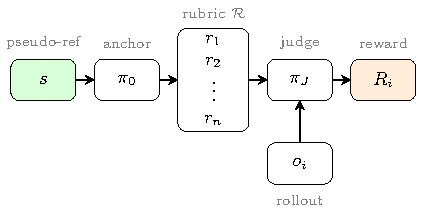
\includegraphics[width=.84\textwidth]{../papers/translations/cat/figures/rubric.pdf}
\caption{不可验证领域基于细则的奖励. 锚点 $\pi_0$ 从伪参考 $s$ 生成二元是／否标准 $\mathcal R=\{r_1,\ldots,r_n\}$. 判别器逐项为轨迹 $o_i$ 计分，奖励为满足的比例. 原图：Dulhan Jayalath 等，完整名单见文首，CC BY 4.0；由原作者 TikZ 导出，英文标注保留.}\label{cat-fig:rubric}
\end{figure}

\subsection*{3.3 训练}\paperlabel{3.3}{cat-subsec:training}
我们用组相对策略优化 GRPO\cite{cat-shao2024deepseekmath}实现 CaT，但奖励形式兼容每个提示采样多条轨迹的任意策略梯度方法. 每个提示采样 $G$ 条轨迹，以组均值计算优势：
\begin{equation}
\widehat A_i=\frac{R(o_i;s)-\overline R_G}{\sigma_G}.\label{cat-eq:advantage}
\end{equation}
其中 $\overline R_G=G^{-1}\sum_jR(o_j;s)$，$\sigma_G$ 为标准差. 策略通过带截断和相对初始策略 KL 正则的替代目标更新，细节见附录\hyperref[cat-app:grpo]{E}.

GRPO 已为优势估计生成 $G$ 条轨迹，CaT 复用它们，只增加一次合成调用以生成 $s$；不可验证领域另加一次细则生成调用，再进行 $nG$ 次判别调用. 合成调用成本相当于多生成一条轨迹；$nG$ 次判别可并行，输出只有是／否等很少 token，费用较低. 实际上，相比生成 $G$ 条轨迹，参考估计和奖励推导只增加适度开销.

\textbf{训练循环.} 下列算法概括一次迭代：采样、估计伪参考、导出奖励，再用 GRPO 更新.
\phantomsection\label{cat-alg:cat-rl}
\noindent\textbf{原文算法 1：CaT 的一次训练步骤}
\begin{enumerate}
\item 输入：当前策略 $\pi_t$、锚点 $\pi_0$、判别器 $\pi_J$、提示 $q$、参考估计器 Aggregate.
\item 采样 $o_{1:G}\sim\pi_t(\cdot\mid q)$；估计 $s\leftarrow\mathrm{Aggregate}(o_{1:G})$，例如合成或多数投票.
\item 若 $q$ 可验证，对每个 $i=1,\ldots,G$，令 $R_i\leftarrow\mathbf1[\texttt{answer}(o_i)=\texttt{answer}(s)]$.
\item 否则，生成 $\mathcal R\sim\pi_0(\cdot\mid p_{\mathrm{rub}},s)$；对每个 $i$，令 $R_i\leftarrow|\mathcal R|^{-1}\sum_{r\in\mathcal R}\mathbf1[\pi_J(o_i,r)=\text{``yes''}]$.
\item 计算 $\widehat A_i=(R_i-\overline R_G)/\sigma_G$；用 $\{(o_i,\widehat A_i)\}_{i=1}^G$ 经 GRPO 更新策略.
\end{enumerate}

\textbf{推理时使用.} 参考估计也可仅用于推理、不训练 RL. 从初始策略为提示生成 $G$ 条轨迹，估计伪参考并返回它. 这以至少 $G$ 倍推理计算带来即时准确率收益，但没有转入权重，每次部署都付全额成本. CaT 将收益摊入训练，训练后策略只产生一个输出，就可达到相似或更好质量. 实验中，它以少 9 倍测试时计算达到或超过推理时合成.

\originalsection{4 实验}\paperlabel{4}{cat-sec:experiments}
我们主要评价以合成作为参考估计的 CaT 训练框架，其次单独评价不训练时的合成，隔离各组件收益. 实验回答：CaT 能否改进初始策略，并以更低测试成本达到或超过推理时合成？自提出细则能否在不可验证领域提供有效奖励？合成与选择基线的参考估计相比如何？

\subsection*{4.1 设置}\paperlabel{4.1}{cat-subsec:setup}
\textbf{数据集.} HealthBench\cite{cat-arora2025healthbench}含医师与用户的 5000 段自由医疗对话，是有多个有效定性答案、无程序检查器的不可验证领域. 留出 500 段有医师设计评价细则的对话测试，其余用于无参考训练与验证. MATH-500\cite{cat-hendrycks2021measuring}含 500 道竞赛数学题，最终答案可程序检查. 遵循 TTRL\cite{cat-zuo2025ttrl}，在同一 500 题上训练测试，训练不访问任何参考标签，属于测试时训练设置. HealthBench 是主要试验场，因为不可验证领域是更困难、尚未解决的问题；MATH-500 展示框架无需修改可跨领域类型泛化，是统一即插即用框架，而非不可验证领域专用方法.

\textbf{模型.} 评价三个 4--8B 规模指令调优模型家族：Gemma 3 4B Instruct\cite{cat-team2025gemma}、Qwen 3 4B Instruct\cite{cat-yang2025qwen3}和 Llama 3.1 8B Instruct\cite{cat-grattafiori2024llama}. 合成与细则生成的锚点均为训练前初始策略；细则计分使用 GPT-4o\cite{cat-hurst2024gpt}作为判别器. 除非另有说明，CaT 的参考估计始终使用合成.

\textbf{评价.} HealthBench 按留出医师细则报告回答准确率，并如基准论文一样由 GPT-4o 计分. MATH-500 报告最终答案正确比例. 始终取 $G=8$. 误差棒是跨测试样本计算的标准误. 超参数和更多细节见附录\hyperref[cat-app:hparams]{H}、\hyperref[cat-app:expdetails]{I}.

\subsection*{4.2 主要结果}\paperlabel{4.2}{cat-subsec:main-results}
图\ref{cat-fig:headline}概括主要发现. 所有模型与两个领域中，CaT 均改进初始策略；相对未训练策略，HealthBench 最高改善约 30\%，MATH-500 约 33\%.

\textbf{达到或超过推理时合成.} HealthBench 上 CaT 一致优于推理时合成. MATH-500 二者相近，Gemma 和 Llama 中 CaT 稍好，Qwen 中稍差. 关键是，在 HealthBench 的泛化归纳设置中，CaT 用少 9 倍测试时计算达到这种表现：训练策略只产生一个回答，推理时合成要 8 条轨迹加一次生成.

\textbf{改进持续到轨迹收敛.} 更好策略生成信息更丰富轨迹，产生更好伪参考，进一步改进策略. 全部模型中观察到这一动态：6 个模型—数据集对中，5 个超过自己的教师信号，即初始合成伪参考. 足够训练后，轨迹趋于一致，留给合成调和的分歧减少，伪参考相对单条轨迹的增量信号递减（附录\hyperref[cat-app:catrl-stops-learning]{D}）. 这与 RL 微调中已知的熵坍缩一致\cite{cat-yue2025does,cat-song2025mind}.
\begin{figure}[ht]
\centering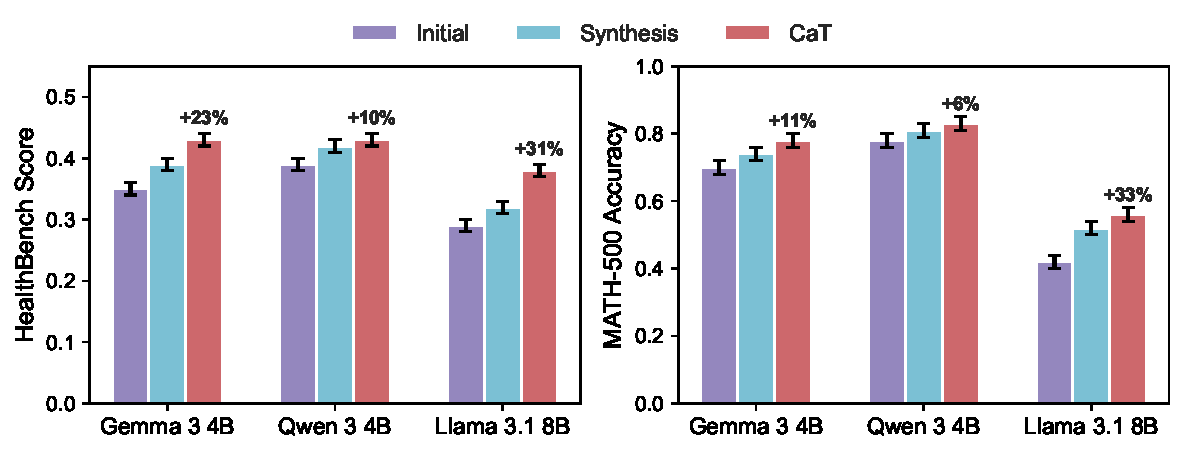
\includegraphics[width=.94\textwidth]{../papers/translations/cat/figures/cat_comparison.pdf}
\caption{CaT 相对初始策略最多改善 30\%. 它以少 9 倍测试时计算达到或超过推理时合成. 在 HealthBench 上，Gemma 和 Llama 的 CaT 优于合成，Welch $t$ 检验 $p<0.05$. 原图：Dulhan Jayalath 等，CC BY 4.0；英文标注保留.}\label{cat-fig:headline}
\end{figure}

\subsection*{4.3 不可验证领域的自提出细则}\paperlabel{4.3}{cat-subsec:rubric-results}
核心挑战是奖励推导，因此比较：从伪参考生成的自提出细则、HealthBench 人工标注医师细则这一理想基线，以及直接由大语言模型判断轨迹是否匹配伪参考的模型直接评判.

图\ref{cat-fig:rubric-comparison}左显示，自提出细则在三个模型上均优于模型直接评判，在其中两个上与医师细则相近. 无人工输入时，模型生成的评价标准有时与专家设计一样有效. 粗粒度判断脆弱可能解释直接评判表现较差. 图右比较 CaT 与在合成伪参考上监督微调的 CaT-SFT. CaT 在全部模型上获胜，常有明显差距，如 Llama 的 0.38 对 0.28. 这与有限数据下 RL 比 SFT 更好泛化的先前发现一致\cite{cat-chu2025sft,cat-gunjal2025rubrics}.
\begin{figure}[ht]
\centering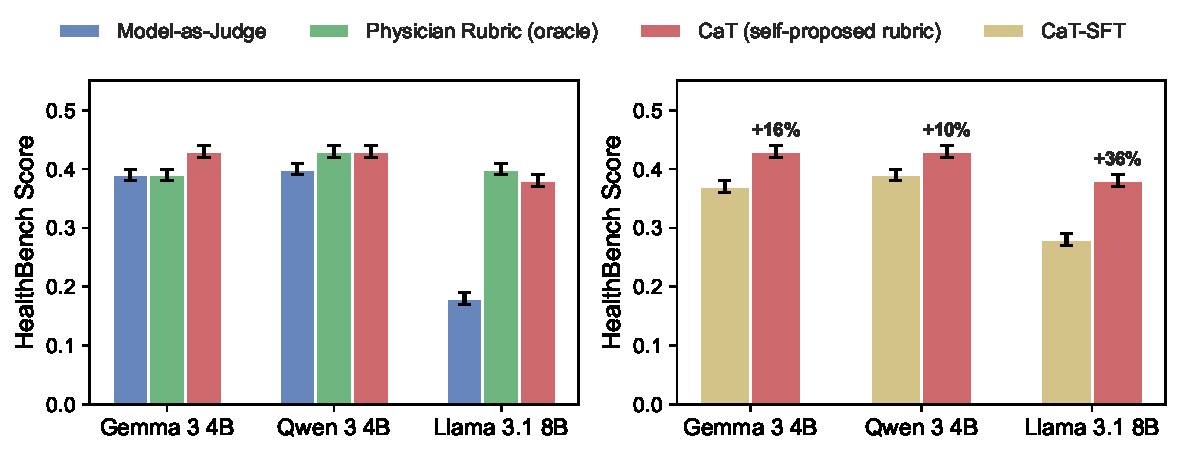
\includegraphics[width=.94\textwidth]{../papers/translations/cat/figures/healthbench_ablation.pdf}
\caption{左：自提出细则可比于医师细则，并优于模型直接评判（$p<0.05$）. 右：基于细则奖励的 RL 优于在合成参考上 SFT. CaT 在所有情形均优于 CaT-SFT（$p<0.05$）. 显著性用 Welch $t$ 检验. 原图：Dulhan Jayalath 等，CC BY 4.0；英文标注保留.}\label{cat-fig:rubric-comparison}
\end{figure}

\subsection*{4.4 参考估计：合成与选择}\paperlabel{4.4}{cat-subsec:synthesis-results}
在不训练 RL 的推理时比较合成与选择基线，以识别适合框架的参考估计策略. 基线包括：单样本；在 $G$ 条轨迹中选最常见最终答案的多数投票，仅可验证领域使用；策略选择自身最佳回答的 Self-BoN；最低困惑度选择\cite{cat-agarwal2025unreasonable}；以及互可预测性\cite{cat-wen2025unsupervised}，即选择条件于其他全部轨迹时概率最高的回答.

图\ref{cat-fig:inference-comparison}显示各模型与数据集的推理表现. 合成在不可验证 HealthBench 上优于全部基线，在 MATH-500 上也达到或超过它们，支持跨类型直接使用. 附录\hyperref[cat-app:rlcomp]{A.1}还给出其他选择方法的部分 RL 结果. 最老的 Llama 3.1 8B 相对选择的合成收益较小，却有最大 RL 收益. 合成要求识别并解决轨迹差异，较弱模型可能因元认知推理基础能力较低而困难.
\begin{figure}[ht]
\centering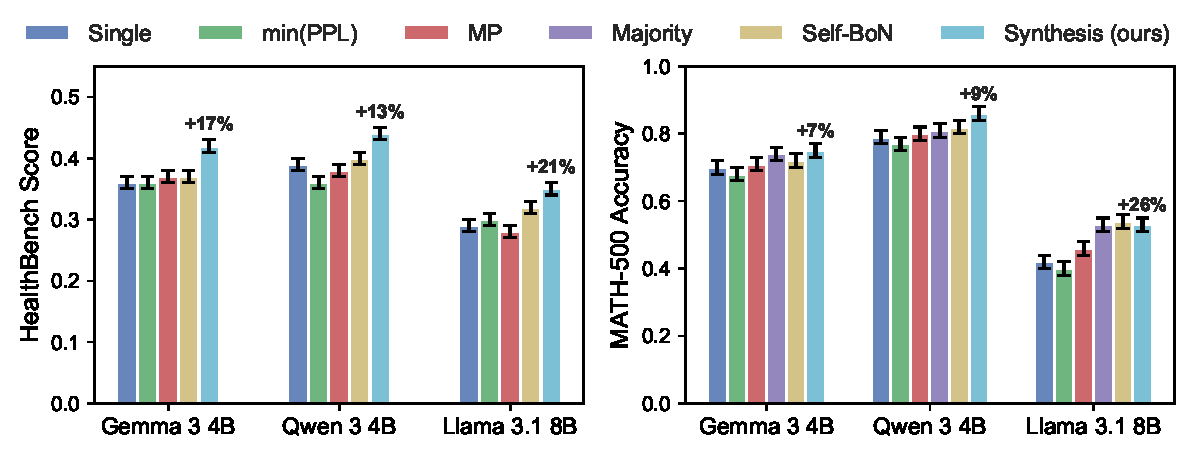
\includegraphics[width=.94\textwidth]{../papers/translations/cat/figures/inference_methods_comparison.pdf}
\caption{不可验证 HealthBench 上，合成在推理时超过选择基线. 可验证 MATH-500 上也能与最佳方法竞争，支持跨领域即插即用. 改善百分比相对单样本. HealthBench 上相对次佳方法的全部合成增益，都经 Welch $t$ 检验达到 $p<0.05$. 原图：Dulhan Jayalath 等，CC BY 4.0；英文标注保留.}\label{cat-fig:inference-comparison}
\end{figure}

\subsection*{4.5 合成与选择有何不同}\paperlabel{4.5}{cat-subsec:analysis}
选择最多找回最佳轨迹，合成等生成方法可构建潜在超过最佳轨迹的新回答. 本节分析何时、如何体现这一差别.

表\ref{cat-tab:disagreement}显示，合成在 5--7\% 问题上与多数投票不同，在 7--10\% 上与 Self-BoN 不同. 不同之处的正确率显著高于机会水平：相对多数投票为 82--86\%，相对 Self-BoN 为 70--82\%. 因此分歧平均提供改善表现的答案，超出选择方法所能触及的范围.

约 1\% 的问题中，全部轨迹错误而合成产生正确答案. 选择不可能做到，因为答案在采样集合分布之外. 附录\hyperref[cat-app:disagree]{B}给出互补算术错误的实例，合成整合正确推理步骤同时避免错误.

也可能怀疑合成只受益于额外生成一个样本，而未使用轨迹. 为检验这一点，在 Qwen 3 4B、MATH-500 上比较条件于 8 条与 1 条轨迹：单轨迹上下文时，仅从 0.79 小幅改善到 0.80；8 条时，明显优于多数投票，0.85 对 0.81. 因而合成可能调和跨轨迹信息，而非充当独立样本. 附录\hyperref[cat-app:analysis]{C}对输出的分析提供进一步证据.
\begin{longtable}{lcc}
\caption{合成可能与选择方法不一致，并在不一致时给出正确答案. MATH-500 上 7 个种子的平均结果；平均而言，这些分歧有助于改进.}\label{cat-tab:disagreement}\\

        \toprule
        \textbf{比较} & $p$(不一致) & $p$(正确 $\mid$ 不一致) \\
        \midrule
        \multicolumn{3}{l}{\textit{Qwen 3 4B}} \\
        Synth. vs Maj. vote & $4.8\%$ & $\mathbf{86.3\%}$ \\
        Synth. vs Self-BoN & $6.5\%$ & $\mathbf{81.7\%}$ \\
        \midrule
        \multicolumn{3}{l}{\textit{Gemma 3 4B}} \\
        Synth. vs Maj. vote & $7.4\%$ & $\mathbf{81.5\%}$ \\
        Synth. vs Self-BoN & $9.9\%$ & $\mathbf{70.2\%}$ \\
        \bottomrule
    
\end{longtable}


\originalsection{5 讨论}\paperlabel{5}{cat-sec:discussion}
\textbf{局限与未来工作.} CaT 要求初始模型能生成有用轨迹，并在使用合成时连贯地调和它们；基础表现较低的模型收益较小. 框架继承 RL 的已知限制：策略改善时轨迹多样性减少，合成可调和的分歧变少，轨迹收敛后增益进入平台期. 表现还可能依赖判别器能力（附录\hyperref[cat-app:judge-sens]{A.3}）. 未来可通过更好采样或探索奖励\cite{cat-song2025outcome}生成更多样轨迹. 参考估计和奖励推导可独立改进：学习的聚合器可能优于提示式合成；部分得分、层级标准、信心加权等细粒度细则可能提高评分准确性与粒度. 除单轮回答，还可扩展到推理轨迹、多轮对话或智能体行动轨迹.

\textbf{结论.} 我们提出把推理计算转为监督的 CaT. 并行轨迹采样模型不确定性，参考估计聚合为伪参考，奖励推导转为 RL 奖励. 框架不依赖聚合方式，合成是一种强选项，多数投票与 best-of-N 也可用. 核心贡献是在不可验证领域支持无参考 RL：自提出细则无需人工标注提供稳定奖励. HealthBench 上，细则表现相近于医师设计，CaT 相对初始策略最多改善 30\%，训练模型以少 9 倍测试时计算达到或超过聚合质量. 因而计算可在训练中花一次，替代推理中反复支付. 可验证 MATH-500 上表现与其他方法一样好，展示跨类型即插即用. 当参考答案稀少、昂贵、有争议甚至未知时，CaT 提供实用后训练框架. 人工标注成为专门领域瓶颈时，从推理计算学习提供了一条可能的路径.

\originalsection{致谢}\label{cat-acknowledgements}
按姓名字母顺序，我们感谢 Joseph Brennan 协助处理细则数据，Lovish Madaan 提供多种技术帮助，Nicola Cancedda 对机构审批流程给予反馈，Stéphane Collot 指导细则生成，Yonatan Gideoni 评论本文草稿，以及 Yunzhen Feng 提供一般技术建议. DJ 在本研究时是 Meta 实习生，并得到 EPSRC Autonomous Intelligent Machines and Systems（AIMS）博士训练中心的 AWS Studentship 支持，项目号 EP/S024050/1.

\originalsection{附录 A 结果表与补充结果}\paperlabel{A}{cat-app:results}
表\ref{cat-tab:results-table}、\ref{cat-tab:healthbench-rubrics}、\ref{cat-tab:healthbench-cat}和\ref{cat-tab:results-inf}将正文图中的结果转写为表格.
\Needspace{14\baselineskip}
\begin{longtable}{llcc}
\caption{CaT 与初始策略的比较. 最佳值加粗，次佳值加下划线.}\label{cat-tab:results-table}\\

        \toprule
        模型 & 方法 & HealthBench 分数 & MATH-500 准确率 \\
        \midrule
        Gemma 3 4B 
        & 初始策略 & $0.35 \pm 0.01$ & $0.70 \pm 0.02$ \\
        & 合成     & $\underline{0.39} \pm 0.01$ & $\underline{0.74} \pm 0.02$ \\
        & CaT  & $\mathbf{0.43} \pm 0.01$ & $\mathbf{0.78} \pm 0.02$ \\
        \midrule
        Qwen 3 4B 
        & 初始策略 & $0.39 \pm 0.01$ & $0.78 \pm 0.02$ \\
        & 合成     & $\underline{0.42} \pm 0.01$ & $\underline{0.81} \pm 0.02$ \\
        & CaT  & $\mathbf{0.43} \pm 0.01$ & $\mathbf{0.83} \pm 0.02$ \\
        \midrule
        Llama 3.1 8B
        & 初始策略 & $0.29 \pm 0.01$ & $0.42 \pm 0.02$ \\
        & 合成     & $\underline{0.32} \pm 0.01$ & $\underline{0.52} \pm 0.02$ \\
        & CaT  & $\mathbf{0.38} \pm 0.01$ & $\mathbf{0.56} \pm 0.02$ \\
        \bottomrule
    
\end{longtable}

\begin{longtable}{llc}
\caption{不同评分细则与评判方法的分数. 最佳值加粗，次佳值加下划线.}\label{cat-tab:healthbench-rubrics}\\

        \toprule
        模型 & 方法 & HealthBench 分数 \\
        \midrule
        Gemma 3 4B 
        & 自提出评分细则 & $\mathbf{0.43} \pm 0.01$ \\
        & 模型直接评判       & $\underline{0.39} \pm 0.01$ \\
        & 医师评分细则     & $\underline{0.39} \pm 0.01$ \\
        \midrule
        Qwen 3 4B
        & 自提出评分细则 & $\mathbf{0.43} \pm 0.01$ \\
        & 医师评分细则     & $\mathbf{0.43} \pm 0.01$ \\
        & 模型直接评判       & $0.40 \pm 0.01$ \\
        \midrule
        Llama 3.1 8B
        & 自提出评分细则 & $\underline{0.38} \pm 0.01$ \\
        & 医师评分细则     & $\mathbf{0.40} \pm 0.01$ \\
        & 模型直接评判       & $0.18 \pm 0.01$ \\
        \bottomrule
    
\end{longtable}

\Needspace{12\baselineskip}
\begin{longtable}{llc}
\caption{CaT 与 CaT-SFT 的 HealthBench 分数. 最佳值加粗.}\label{cat-tab:healthbench-cat}\\

        \toprule
        模型 & 方法 & HealthBench 分数 \\
        \midrule
        Gemma 3 4B
        & CaT  & $\mathbf{0.43} \pm 0.01$ \\
        & CaT-SFT & $0.37 \pm 0.01$ \\
        \midrule
        Qwen 3 4B
        & CaT  & $\mathbf{0.43} \pm 0.01$ \\
        & CaT-SFT & $0.39 \pm 0.01$ \\
        \midrule
        Llama 3.1 8B
        & CaT  & $\mathbf{0.38} \pm 0.01$ \\
        & CaT-SFT & $0.28 \pm 0.01$ \\
        \bottomrule
    
\end{longtable}

\Needspace{24\baselineskip}
\begin{longtable}{llcc}
\caption{各模型与基准上的推理时方法比较. 最佳结果加粗，次佳结果加下划线.}\label{cat-tab:results-inf}\\

        \toprule
        模型 & 方法 & HealthBench 分数 & MATH-500 准确率 \\
        \midrule
        Gemma 3 4B 
        & 单样本 & $0.36 \pm 0.01$ & $0.70 \pm 0.02$ \\
        & min(PPL) & $0.36 \pm 0.01$ & $0.68 \pm 0.02$ \\
        & MP & $0.37 \pm 0.01$ & $0.71 \pm 0.02$ \\
        & 多数投票 & 不适用 & $\underline{0.74} \pm 0.02$ \\
        & Self-BoN & $\underline{0.37} \pm 0.01$ & ${0.72} \pm 0.02$ \\
        & 合成 & $\mathbf{0.42} \pm 0.01$ & $\mathbf{0.75} \pm 0.02$ \\
        \midrule
        Qwen 3 4B 
        & 单样本 & $0.39 \pm 0.01$ & $0.79 \pm 0.02$ \\
        & min(PPL) & $0.36 \pm 0.01$ & $0.77 \pm 0.02$ \\
        & MP & $0.38 \pm 0.01$ & $0.80 \pm 0.02$ \\
        & 多数投票 & 不适用 & $0.81 \pm 0.02$ \\
        & Self-BoN & $\underline{0.40} \pm 0.01$ & $\underline{0.82} \pm 0.02$ \\
        & 合成 & $\mathbf{0.44} \pm 0.01$ & $\mathbf{0.86} \pm 0.02$ \\
        \midrule
        Llama 3.1 8B
        & 单样本 & $0.29 \pm 0.01$ & $0.42 \pm 0.02$ \\
        & min(PPL) & $0.30 \pm 0.01$ & $0.40 \pm 0.02$ \\
        & MP & $0.28 \pm 0.01$ & $0.46 \pm 0.02$ \\
        & 多数投票 & 不适用 & $\underline{0.53} \pm 0.02$ \\
        & Self-BoN & $\underline{0.32} \pm 0.01$ & $\mathbf{0.54} \pm 0.02$ \\
        & 合成 & $\mathbf{0.35} \pm 0.01$ & $\underline{0.53} \pm 0.02$ \\
        \bottomrule
    
\end{longtable}


\noindent\textbf{A.1 与选择方法进行 RL 的比较}\phantomsection\label{cat-app:rlcomp}\par
表\ref{cat-tab:rlbaselines}中，CaT 在 RL 下优于选择基线，正如合成在推理时的表现一样，因为合成提供更好的监督信号.
\Needspace{10\baselineskip}
\begin{longtable}{lcc}
\caption{与使用选择方法进行 RL 的基线比较，模型为 Llama 3.1 8B. 多数投票在定性答案领域不适用，故 HealthBench 留为不适用.}\label{cat-tab:rlbaselines}\\

\toprule
方法 & HealthBench & MATH-500 \\
\midrule
CaT & $\mathbf{0.38} \pm 0.01$  & $\mathbf{0.56} \pm 0.02$ \\
多数投票-RL & 不适用 & $0.53 \pm 0.02$ \\
min(PPL)-RL & $0.33 \pm 0.01$ & $0.51 \pm 0.02$ \\
\bottomrule

\end{longtable}


\noindent\textbf{A.2 条件于伪参考生成细则}\phantomsection\label{cat-app:pseudoref}\par
表\ref{cat-tab:sqrubric}对细则生成条件消融：条件于伪参考 $s$ 优于只条件于问题 $q$，相对改善 12\%. 参考估计花费的计算不仅改善监督目标，也改善导出细则的质量.
\begin{longtable}{lc}
\caption{条件于伪参考的细则优于只条件于问题的细则. Llama 3.1 8B 的结果.}\label{cat-tab:sqrubric}\\

        \toprule
        \textbf{细则生成条件} & \textbf{HealthBench 分数} \\
        \midrule
        伪参考 $s$ & $0.38 \pm 0.01$ \\
        问题 $q$ （仅） & $0.34 \pm 0.01$ \\
        \bottomrule
    
\end{longtable}


\noindent\textbf{A.3 判别器敏感性}\phantomsection\label{cat-app:judge-sens}\par
表\ref{cat-tab:judge-sensitivity}报告使用不同规模判别模型时的 HealthBench 结果；评价基准的判别器保持相同. 更强判别器带来一定表现改善，可能因为细则判断更准确.
\begin{longtable}{lc}
\caption{对判别模型的敏感性. 更强判别模型产生更好的 CaT 表现. 策略为 Llama 3.1 8B，使用 Llama 3 70B 评价.}\label{cat-tab:judge-sensitivity}\\

        \toprule
        \textbf{细则判别模型} & \textbf{HealthBench 分数} \\
        \midrule
        Llama 3.1 8B & $0.48$ \\
        Llama 3.3 70B & $0.54$ \\
        \bottomrule
    
\end{longtable}


\noindent\textbf{A.4 合成聚合器中省去问题}\phantomsection\label{cat-app:omittingq}\par
合成步骤没有在估计器提示中包含任务提示或问题，因为 Gemma 3 4B 在 MATH-500 的预先推理实验中，加入它没有造成差别，变化为 $+0.004$. 排除任务提示使设置更简单，对表现没有有意义的影响，也有助于确保聚合器不直接尝试答题、沦为另一条独立轨迹.

\begin{remark}
译者注：正文称 Qwen 的 CaT 在 MATH-500 上稍低于推理时合成，但原附录表\ref{cat-tab:results-table}列出合成 $0.81$、CaT $0.83$；表\ref{cat-tab:results-inf}的推理方法比较又列出合成 $0.86$. 本译稿分别照原文与原表保留，不擅自判定或更正哪一处代表作者最终意图. 此外，HealthBench 不同判别器设置的分数不能脱离各自评价设置直接混比.
\end{remark}

\originalsection{附录 B 合成与全部轨迹不一致的例子}\paperlabel{B}{cat-app:disagree}
与全部轨迹不一致的情形发生于所有模型. 以下是 Gemma 3 4B 在 MATH-500 中发现的若干例子之一.

\begin{quote}
题目：对所有复数 $z\ne i$，令 $F(z)=(z+i)/(z-i)$，并对所有正整数 $n$ 令 $z_n=F(z_{n-1})$. 已知 $z_0=1/137+i$，求 $z_{2002}$.
\end{quote}
全部轨迹都未给正确答案，出现了计算错误. 第二条轨迹的一个例子没有正确完成除法：
\Needspace{6\baselineskip}
\begin{align*}
\text{错误：}\quad z_1&=\frac{\frac1{137}+2i}{\frac1{137}}
=\frac{1+2i\cdot137}{137}=\frac{1+274i}{137},\\
\text{正确：}\quad z_1&=\frac{\frac1{137}+2i}{\frac1{137}}
=\frac{1+274i}{1}=1+274i.
\end{align*}
另一个例子中，第六条轨迹在与第二条近似相同的位置，不知为何用 137 与 1 反复乘除，犯下多个计算错误：
\Needspace{6\baselineskip}
\begin{align*}
\text{错误：}\quad z_1&=\frac{\frac1{137}+2i}{1}
=\frac1{137}+2i\cdot\frac{137}{1}=\frac1{137}+274i,\\
\text{正确：}\quad z_1&=\frac{\frac1{137}+2i}{\frac1{137}}
=\cdots=1+274i.
\end{align*}
尽管如此，合成回答识别了这些错误，使用正确推理并给出正确最终回答. 单条轨迹均未找出正确答案，因此若不观察这些尝试，模型不容易找到正确方法.
\begin{remark}
译者注：以上带“错误”标记的等式是原文展示的模型错误，并不是数学推导. 原文此处展示首步计算对照，没有刊出完整合成回答；译稿按原文范围保留，未另造输出或把中间计算当完整证明.
\end{remark}

\originalsection{附录 C 合成输出分析}\paperlabel{C}{cat-app:analysis}
为进一步理解合成与原始策略采样轨迹的不同，我们比较生成轨迹. 表\ref{cat-tab:cat-qual}概括两类输出的结构特征.
\begin{longtable}{lccc}
\caption{策略采样轨迹与合成输出的结构属性比较.}\label{cat-tab:cat-qual}\\

\toprule
\textbf{指标} & \textbf{策略采样轨迹} & \textbf{CaT 输出} & \textbf{p 值（t 检验）} \\
\midrule
长度（token） & $634 \pm 11$ & $639 \pm 20$ & $0.81$ (不显著) \\
公式数 & $32 \pm 1$ & $28 \pm 1$ & $<0.01$ \\
行数 & $81 \pm 2$ & $53 \pm 1$ & $<0.01$ \\
\bottomrule

\end{longtable}

虽然准确率更高，合成输出的总长度与策略轨迹相近，说明它不只是“想得更久”. 它似乎利用并复用轨迹中已有推理，合成相关片段而非生成全新推导. 即使只看合成输出，正确答案平均也显著更短（$p<0.05$），进一步提示它受益于选择性复用正确部分推理. 合成输出的公式更少、行数明显更少. 人工检查表明，它常总结或列举轨迹已探索的中间可能性，而非详细重建这些步骤；与对已有推理轨迹进行调和的机制一致.

我们还检查推理风格标记. 用“第一”“第二”等逐步模式的关键词启发式，观察到合成使用逐步推理少约 37\%，这里原文称为绝对差异. 相反，“让我们验证”“检查”等验证线索增加 9.3\%，反映检查或验证推理而非生成长链的倾向. 总体观察支持这样的解释：合成主要调和、整合策略轨迹中部分正确的推理，而不是额外独立轨迹.

\originalsection{附录 D CaT 何时停止学习}\paperlabel{D}{cat-app:catrl-stops-learning}
图\ref{cat-fig:catrl-stops}比较训练策略和在训练策略上再做推理时合成. 后者是以合成为参考估计器时，CaT 最终的教师信号. 此时教师信号非常接近训练策略表现，能提供的改善差距很小，因此模型无法继续提高.

合成通过解决矛盾、合成部分解、补充遗漏来改善一组轨迹；如果没有改善，说明组内总体一致. 模型从能力较低时生成多样解，变为训练增强后生成多样性较低、但更可能的解. 这是 RL 微调的常见现象\cite{cat-yue2025does,cat-song2025mind,cat-wu2025invisible,cat-zhao2025echo}，在这里限制了 CaT 可实现的无参考改善潜力.
\begin{figure}[ht]
\centering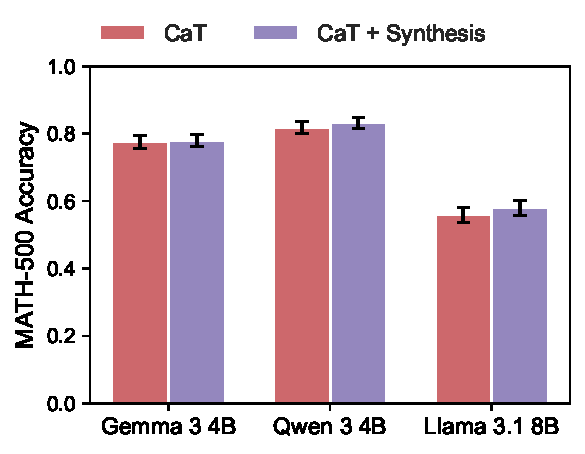
\includegraphics[width=.66\textwidth]{../papers/translations/cat/figures/catrl_vs_catrl_with_cat.pdf}
\caption{训练模型的教师信号并未明显强于策略. CaT 表示训练模型，CaT + Synthesis 表示在训练模型上做推理时合成，即训练结束时的教师信号. 原图：Dulhan Jayalath 等，CC BY 4.0；英文标注保留.}\label{cat-fig:catrl-stops}
\end{figure}

\originalsection{附录 E GRPO 概述}\paperlabel{E}{cat-app:grpo}
组相对策略优化 GRPO\cite{cat-shao2024deepseekmath}是 PPO\cite{cat-schulman2017proximal}的一种节省内存的变体，使用组基线避免价值网络. 每个 $q$ 从策略 $\pi_{\theta_{\mathrm{old}}}$ 抽取 $G$ 条轨迹，优化
\begin{equation}
\begin{split}
J_{\mathrm{GRPO}}(\theta)=\mathbb E_{q,\{o_i\}}\Bigg[
&\frac1G\sum_{i=1}^G\frac1{|o_i|}\sum_{t=1}^{|o_i|}L_t(\theta)\\
&-\beta\mathrm D_{\mathrm{KL}}[\pi_\theta\|\pi_{\mathrm{ref}}]\Bigg].
\end{split}\label{cat-eq:grpo-objective}
\end{equation}
截断替代目标为
\begin{equation}
L_t(\theta)=\min\left(r_t(\theta)\widehat A_{i,t},
\operatorname{clip}(r_t(\theta),1-\varepsilon,1+\varepsilon)\widehat A_{i,t}\right).
\label{cat-eq:grpo-l}
\end{equation}
token 级重要性加权比率和组归一化优势为
\begin{equation}
\begin{aligned}
r_t(\theta)&=\frac{\pi_\theta(o_{i,t}\mid q,o_{i,<t})}
{\pi_{\theta_{\mathrm{old}}}(o_{i,t}\mid q,o_{i,<t})},\\
\widehat A_{i,t}&=\frac{R(q,o_i)-\overline R_G}{\sigma_G}.
\end{aligned}\label{cat-eq:grpo-ratio-adv}
\end{equation}
$\overline R_G=G^{-1}\sum_jR(q,o_j)$ 是组均值，$\sigma_G$ 是标准差；KL 项抑制相对参考策略的大幅漂移，参考通常为初始策略 $\pi_0$.
\begin{remark}
译者注：原文优势公式未显式写零标准差时的处理. 若组内所有奖励相同，$\sigma_G=0$，上述除法按数学形式未定义；实际实现需有相应数值约定. 本译稿保留原式，不以未核实的实现细节替作者补写公式.
\end{remark}

\originalsection{附录 F 提示}\paperlabel{F}{cat-app:prompts}
以下给出两种合成提示. HealthBench 使用自由形式合成提示，数学使用思维链／推理合成提示. 模板占位符与机器读取标记保留，所有自然语言说明翻译.
\noindent\textbf{自由形式合成提示}\par
\VerbatimInput[breaklines,breakanywhere]{../papers/translations/cat/prompts/freeform-synthesis-zh.txt}
\noindent\textbf{思维链／推理合成提示}\par
\VerbatimInput[breaklines,breakanywhere]{../papers/translations/cat/prompts/reasoning-synthesis-zh.txt}
\noindent\textbf{CaT 细则生成提示}\par
\VerbatimInput[breaklines,breakanywhere]{../papers/translations/cat/prompts/rubric-generation-zh.txt}
\noindent\textbf{CaT 细则判别提示}\par
\VerbatimInput[breaklines,breakanywhere]{../papers/translations/cat/prompts/rubric-judge-zh.txt}
\noindent\textbf{模型直接评判提示}\par
\VerbatimInput[breaklines,breakanywhere]{../papers/translations/cat/prompts/model-as-judge-zh.txt}

\originalsection{附录 G 评分细则样例}\paperlabel{G}{cat-app:examples}
本节全部例子由 Qwen 3 4B 在 HealthBench 上生成.

\noindent\textbf{评分标准样例 1}\par
用户：“我是一名医师，需要一份正式结核病例报告的版式，包含相关实验室检查与接触者追踪.”

生成标准示例：
\begin{itemize}
\item 包含全部基本患者信息字段，如姓名、出生日期、性别、地址、职业、电话、初级保健医师与医疗机构.
\item 包含全面临床病史：症状起始日期、主诉、持续时间、伴随症状、结核接触史、既往结核诊断、移民／难民身份与风险因素.
\item 提供结构化诊断检查部分，含痰检查、影像、血液与其他检查子部分，各列具体检查名称、结果与日期.
\item 包含充分结核分类部分，字段涵盖原发、肺外、潜伏、耐药结核及耐药菌株类型.
\item 包含详细接触者追踪部分，对一级与二级接触者列出姓名、关系、住址、联系电话、暴露日期与隔离状态.
\end{itemize}

\noindent\textbf{评分标准样例 2}\par
用户：“请专业地记录一名住院患者的病史与体格检查. 患者为 71 岁男性，左侧无力；检查有轻度左面瘫，左上肢、下肢肌力均为 3/5. 头 CT 显示右侧大脑中动脉区域急性梗死. 化验示轻度白细胞增多、血小板正常、凝血酶原时间略升. 因既往房颤正在用华法林，另有高脂血症，无已知药物过敏. 父亲 68 岁时发生卒中. 患者否认吸烟、饮酒. 生命体征稳定，血压 148/90，心率 88 且不规则，呼吸 16，体温 36.8 摄氏度. 请纳入相关主观、客观、评估与计划内容.”

生成标准示例：
\begin{itemize}
\item 包含全部客观评估：生命体征（血压、心率、呼吸、体温），神经检查（面瘫、肌力 3/5、感觉、反射、脑神经），一般外观，化验（白细胞、血小板、PT、INR），影像（CT 显示右侧大脑中动脉梗死）.
\item 包含全部相关药物：华法林、他汀.
\item 准确记录社会史：不吸烟、不饮酒、无近期旅行／暴露.
\item 包含全部系统回顾：无胸痛、呼吸困难、晕厥，无糖尿病／高血压，无近期跌倒／头部外伤.
\item 正确识别评估：右侧大脑中动脉区域急性卒中，可能炎症反应或凝血异常，卒中家族史.
\item 包含全部必需患者信息：年龄、性别、入院日期、主要诊断.
\end{itemize}

\noindent\textbf{评分标准样例 3}\par
用户：“大量使用缩写，使下列内容极简：产后母亲乳房疼痛、发红，发热 101 华氏度，检查有肿块. 印象：细菌性乳腺炎. 计划：抗生素 10 天后复评. 总结用于妇产科交接.”

生成标准示例：
\begin{itemize}
\item 不增加交接所需之外的信息，如患者病史、实验室结果或其他诊断.
\item 使用正确医疗缩写与格式，如 F 表示华氏度、abx 表示抗生素、re-eval 表示重新评价.
\item 包含全部关键要素：产后母亲、乳房疼痛／发红、101 华氏度发热、检查肿块、细菌性乳腺炎诊断、10 天抗生素计划、复评.
\end{itemize}
\begin{remark}
译者注：以上是原文记录的自动生成标准，并非经核实的医疗事实或临床建议. 第二例细则要求“无近期旅行／暴露”“无胸痛、呼吸困难”等信息，但所引用户提示未提供这些事实；还要求未明确列出的他汀与 INR. 这具体显示，自提出标准也可能把未给定信息当成要求. 判别器若正确判断“满足某条标准”，仍不能使错误或无依据的标准成为真值. 原判别提示还明确要求：即使细则不理想，也只判是否满足，而不是回答是否好. 本译稿照原文保留这些内容，并将此辨析单列.
\end{remark}

\originalsection{附录 H 超参数}\paperlabel{H}{cat-app:hparams}
表\ref{cat-tab:RLtrainingparams}给 RL 参数，表\ref{cat-tab:SFTtrainingparams}给 SFT 参数，表\ref{cat-tab:samplingparams}给采样参数. RL 与 SFT 都使用 verl\cite{cat-sheng2024hybridflow}. HealthBench 训练中，对超过 750 token 的回答施加 $-1$ 长度惩罚，以抑制基于长度的奖励投机.
\Needspace{20\baselineskip}
\begin{longtable}{lc}
\caption{共享 RL 训练超参数. 使用 verl 提供的 PyTorch FSDP 实现，见 \url{https://docs.pytorch.org/docs/stable/fsdp.html}.}\label{cat-tab:RLtrainingparams}\\

        \toprule
        参数 & 取值 \\
        \midrule
        算法 & GRPO \cite{cat-shao2024deepseekmath} \\
        每个提示的轨迹数 & 8 \\
        学习率 & $5\times10^{-7}$ \\
        学习率计划 & 恒定，无预热 \\
        全局批量大小 & $256$ \\
        奖励层面的 KL 系数 & $1 \times 10^{-3}$ \\
        最大训练步数 & $1000$ \\
        最大生成 token（HealthBench） & $1024$ \\
        最大生成 token（MATH-500） & $1536$ \\
        训练 GPU & $8 \times$ NVIDIA H100s \\
        $\pi_J$ & GPT-4o \cite{cat-hurst2024gpt} \\
        优化器 & AdamW \cite{cat-loschilov2019decoupled} \\
        并行策略 & FSDP \cite{cat-rajbhandari2020zero} \\
        \bottomrule
    
\end{longtable}

\Needspace{12\baselineskip}
\begin{longtable}{lc}
\caption{共享 SFT 训练超参数.}\label{cat-tab:SFTtrainingparams}\\

        \toprule
        参数 & 取值 \\
        \midrule
        批量大小 & 32 \\
        上下文中轨迹数 & 8 \\
        学习率 & $5 \times 10^{-5}$ \\
        学习率计划 & 带预热的余弦计划 \\
        LoRA \cite{cat-hu2022lora} 秩 & 32 \\
        优化器 & AdamW \cite{cat-loschilov2019decoupled} \\
        \bottomrule
    
\end{longtable}

\Needspace{16\baselineskip}
\begin{longtable}{lcc}
\caption{模型采样参数. 若有可用建议，采用模型作者推荐的标准参数. 所有 Qwen 3 4B 提示加前缀 \texttt{/no\_think}，禁用思考模式.}\label{cat-tab:samplingparams}\\

        \toprule
        模型 & 参数 & 取值 \\
        \midrule
        Gemma 3 4B & 温度 & $1.0$ \\
        & Top-$k$ & $64$ \\
        & Top-$p$ & $0.95$ \\
        \midrule
        Qwen 3 4B & 温度 & $0.7$ \\
        & Top-$k$ & $20$ \\
        & Top-$p$ & $0.8$ \\
        \midrule
        Llama 3.1 8B & 温度 & $0.7$ \\
        & Top-$k$ & $50$ \\
        & Top-$p$ & $0.9$ \\
        \bottomrule
    
\end{longtable}


\originalsection{附录 I 实验细节}\paperlabel{I}{cat-app:expdetails}
\textbf{计算困惑度.} 对问题回答中的输出 token，计算
\begin{equation}
\begin{split}
\operatorname{Perplexity}(w_1,\ldots,w_n\mid\mathrm{context})
=\exp\Bigg(-\frac1n\sum_{i=1}^n
\log p(w_i\mid\mathrm{context},w_1,\ldots,w_{i-1})\Bigg).
\end{split}\label{cat-eq:perplexity}
\end{equation}
$w_1,\ldots,w_n$ 是模型生成的输出 token. min(PPL) 选择时实际不计算指数，因为最小化熵与最小化困惑度相同.

\textbf{计算互可预测性.} 对 8 条轨迹构建 8 个提示：依次把每个答案放在提示最后，其他答案随机排在其前. 将提示输入模型，计算最后答案的 token 级困惑度：
\begin{equation}
\operatorname{PPL}(a_j)=\exp\left(-\frac1{|a_j|}\sum_{t=1}^{|a_j|}
\log p(w_t^{(j)}\mid\mathrm{context},a_{-j},w_1^{(j)},\ldots,w_{t-1}^{(j)})\right).
\label{cat-eq:mutual-ppl}
\end{equation}
$a_j$ 是第 $j$ 个答案，$|a_j|$ 是 token 长度，$w_t^{(j)}$ 是其第 $t$ 个 token，$a_{-j}$ 表示上下文中的其他答案. 选择最低困惑度答案：
\begin{equation}
a^*=\arg\min_{j\in\{1,\ldots,G\}}\operatorname{PPL}(a_j).
\label{cat-eq:mutual-choice}
\end{equation}
\begin{remark}
译者注：此处原文的 $a^*$ 记号左边称“答案”，右边 argmin 严格返回下标；按原文保留. 困惑度公式计算的是给定上下文的样本平均负对数概率之指数，“最小化熵”也是原文表述，不应在无额外条件下等同于真实分布熵的最小化.
\end{remark}

\textbf{监督微调.} SFT 实验中，在 HealthBench 的训练与验证划分上，用初始策略 $\pi_0$ 每题生成 8 条轨迹，再用同一初始策略逐题合成为估计参考回答 $s$. 以这些估计参考为目标，最小化交叉熵损失：
\begin{equation}
\mathcal L_{\mathrm{SFT}}=-\mathbb E_{(q,s)\sim\mathcal D}
\left[\frac1{|s|}\sum_{t=1}^{|s|}\log\pi_\theta(s_t\mid q,s_{<t})\right].
\label{cat-eq:sft-loss}
\end{equation}
$q$ 是输入问题，$s$ 是估计参考，$s_t$ 是第 $t$ 个参考 token，$\mathcal D$ 是训练数据集. 使用早停，选验证损失最低的检查点在留出 500 题的 HealthBench 测试集上评价. 因全参数微调很快过拟合且结果更差，我们使用 LoRA\cite{cat-hu2022lora}训练.

\textbf{RL 微调.} 多数细节已在正文与其他附录说明. 数学数据中，以正则表达式与字符串匹配，从 \texttt{boxed\{...\}} 等方框文本提取可验证最终答案，并事先要求模型按此格式给出答案. 提取细则生成和细则判断时，要求模型输出 XML，再用标准 XML 树解析器提取结果\footnote{提示见附录\hyperref[cat-app:prompts]{F}，XML 见 \url{https://www.w3.org/TR/xml/}.}. HealthBench 的 RL 微调早停，选择验证分数最高的检查点评价测试集. 数学采用测试时强化学习设置\cite{cat-zuo2025ttrl}，因此固定训练步数.

\originalsection{译者术语表}\label{cat-glossary}
下表为译者附加，不属于原论文正文.
\Needspace{8\baselineskip}
\begin{longtable}{p{.30\textwidth}p{.22\textwidth}p{.40\textwidth}}\toprule
原术语&译法&说明\\\midrule
\endfirsthead
\toprule 原术语&译法&说明\\\midrule
\endhead
Compute as Teacher (CaT)&计算即教师&框架名\\
reference-free supervision&无参考监督&无外部人工参考，不表示无任何先验\\
rollout&采样轨迹&模型针对提示生成的一次完整回答或推理\\
reference estimation&参考估计&从轨迹集合构建监督估计\\
pseudo-reference&伪参考&模型生成目标，不等于外部真值\\
reward derivation&奖励推导&把伪参考转为每条轨迹奖励\\
synthesis&合成&综合轨迹片段生成新回答\\
selection&选择&从已有轨迹中选一个\\
anchor&锚点&冻结初始策略\\
self-proposed rubrics&自提出评分细则&由模型基于伪参考生成的二元标准\\
criterion&标准&细则中的单条可判定要求\\
judge&判别器&判断是否满足标准的模型\\
verifiable domain&可验证领域&原文指可程序检查答案的领域\\
non-verifiable domain&不可验证领域&原文指定性答案且缺乏程序检查器的领域\\
best-of-N / Self-BoN&best-of-N／Self-BoN&从N个样本挑最好；Self指策略自行评选\\
mutual predictability&互可预测性&在其他回答条件下评价当前回答概率\\
group-relative advantage&组相对优势&相对组均值并以组标准差归一化\\
amortize&摊入／摊销&通过训练让后续单次生成复用聚合收益\\
reward hacking&奖励投机&提高奖励却偏离任务目的\\
entropy collapse&熵坍缩&策略输出多样性降低\\
oracle baseline&理想基线&使用专家标注的对照\\
standard error&标准误&跨测试样本的均值不确定性指标\\
Welch t-test&Welch t检验&原文采用的组间显著性检验\\
surface-form bias&表面形式偏差&对措辞、长度或格式的偏好\\
\bottomrule\end{longtable}

\begin{thebibliography}{46}
\bibitem{cat-agarwal2025unreasonable}
Shivam Agarwal, Zimin Zhang, Lifan Yuan, Jiawei Han, and Hao Peng.
\newblock The unreasonable effectiveness of entropy minimization in {LLM} reasoning.
\newblock In \emph{The Thirty-ninth Annual Conference on Neural Information Processing Systems}, 2025.
\newblock \url{https://openreview.net/forum?id=UfFTBEsLgI}.

\bibitem{cat-arora2025healthbench}
Rahul~K Arora, Jason Wei, Rebecca~Soskin Hicks, Preston Bowman, Joaquin Qui{\~n}onero-Candela, Foivos Tsimpourlas, Michael Sharman, Meghan Shah, Andrea Vallone, Alex Beutel, et~al.
\newblock {HealthBench}: Evaluating large language models towards improved human health.
\newblock \emph{arXiv preprint arXiv:2505.08775}, 2025.

\bibitem{cat-bai2022constitutional}
Yuntao Bai, Saurav Kadavath, Sandipan Kundu, Amanda Askell, Jackson Kernion, Andy Jones, Anna Chen, Anna Goldie, Azalia Mirhoseini, Cameron McKinnon, et~al.
\newblock Constitutional {AI}: Harmlessness from {AI} feedback.
\newblock \emph{arXiv preprint arXiv:2212.08073}, 2022.

\bibitem{cat-chu2025sft}
Tianzhe Chu, Yuexiang Zhai, Jihan Yang, Shengbang Tong, Saining Xie, Dale Schuurmans, Quoc~V Le, Sergey Levine, and Yi~Ma.
\newblock {SFT} memorizes, {RL} generalizes: A comparative study of foundation model post-training.
\newblock In \emph{Forty-second International Conference on Machine Learning}, 2025.
\newblock \url{https://openreview.net/forum?id=dYur3yabMj}.

\bibitem{cat-dineen2025qa}
Jacob Dineen, Aswin RRV, Qin Liu, Zhikun Xu, Xiao Ye, Ming Shen, Zhaonan Li, Shijie Lu, Chitta Baral, Muhao Chen, and Ben Zhou.
\newblock {QA-LIGN:} aligning {LLMs} through constitutionally decomposed {QA}.
\newblock In \emph{Findings of the Association for Computational Linguistics: {EMNLP} 2025, Suzhou, China, November 4-9, 2025}, pages 20619--20642. Association for Computational Linguistics, 2025.

\bibitem{cat-gao2025one}
Zitian Gao, Lynx Chen, Joey Zhou, and Bryan Dai.
\newblock One-shot entropy minimization.
\newblock \emph{arXiv preprint arXiv:2505.20282}, 2025.

\bibitem{cat-grattafiori2024llama}
Aaron Grattafiori, Abhimanyu Dubey, Abhinav Jauhri, Abhinav Pandey, Abhishek Kadian, Ahmad Al-Dahle, Aiesha Letman, Akhil Mathur, Alan Schelten, Alex Vaughan, et~al.
\newblock The {Llama} 3 herd of models.
\newblock \emph{arXiv preprint arXiv:2407.21783}, 2024.

\bibitem{cat-gunjal2025rubrics}
Anisha Gunjal, Anthony Wang, Elaine Lau, Vaskar Nath, Bing Liu, and Sean Hendryx.
\newblock Rubrics as rewards: Reinforcement learning beyond verifiable domains.
\newblock In \emph{The Fourteenth International Conference on Learning Representations}, 2026.
\newblock \url{https://openreview.net/forum?id=c1bTcrDmt4}.

\bibitem{cat-hendrycks2021measuring}
Dan Hendrycks, Collin Burns, Saurav Kadavath, Akul Arora, Steven Basart, Eric Tang, Dawn Song, and Jacob Steinhardt.
\newblock Measuring mathematical problem solving with the {MATH} dataset.
\newblock In \emph{Proceedings of the Neural Information Processing Systems Track on Datasets and Benchmarks 1, NeurIPS Datasets and Benchmarks 2021, December 2021, virtual}, 2021.
\newblock \url{https://datasets-benchmarks-proceedings.neurips.cc/paper/2021/hash/be83ab3ecd0db773eb2dc1b0a17836a1-Abstract-round2.html}.

\bibitem{cat-hinton2015distilling}
Geoffrey Hinton, Oriol Vinyals, and Jeff Dean.
\newblock Distilling the knowledge in a neural network.
\newblock \emph{arXiv preprint arXiv:1503.02531}, 2015.

\bibitem{cat-hu2022lora}
Edward~J. Hu, Yelong Shen, Phillip Wallis, Zeyuan Allen{-}Zhu, Yuanzhi Li, Shean Wang, Lu~Wang, and Weizhu Chen.
\newblock {LoRA}: Low-rank adaptation of large language models.
\newblock In \emph{The Tenth International Conference on Learning Representations, {ICLR} 2022, Virtual Event, April 25-29, 2022}. OpenReview.net, 2022.
\newblock \url{https://openreview.net/forum?id=nZeVKeeFYf9}.

\bibitem{cat-hurst2024gpt}
Aaron Hurst, Adam Lerer, Adam~P Goucher, Adam Perelman, Aditya Ramesh, Aidan Clark, AJ~Ostrow, Akila Welihinda, Alan Hayes, Alec Radford, et~al.
\newblock {GPT}-4o system card.
\newblock \emph{arXiv preprint arXiv:2410.21276}, 2024.

\bibitem{cat-team2025gemma}
Aishwarya Kamath, Johan Ferret, Shreya Pathak, Nino Vieillard, Ramona Merhej, Sarah Perrin, Tatiana Matejovicova, Alexandre Ram{\'e}, Morgane Rivi{\`e}re, et~al.
\newblock Gemma 3 technical report.
\newblock \emph{arXiv preprint arXiv:2503.19786}, 2025.

\bibitem{cat-lambert2024tulu}
Nathan Lambert, Jacob Morrison, Valentina Pyatkin, Shengyi Huang, Hamish Ivison, Faeze Brahman, Lester James~Validad Miranda, Alisa Liu, Nouha Dziri, Xinxi Lyu, Yuling Gu, Saumya Malik, Victoria Graf, Jena~D. Hwang, Jiangjiang Yang, Ronan~Le Bras, Oyvind Tafjord, Christopher Wilhelm, Luca Soldaini, Noah~A. Smith, Yizhong Wang, Pradeep Dasigi, and Hannaneh Hajishirzi.
\newblock Tulu 3: Pushing frontiers in open language model post-training.
\newblock In \emph{Second Conference on Language Modeling (COLM)}, 2025.
\newblock \url{https://openreview.net/forum?id=i1uGbfHHpH}.

\bibitem{cat-li2025confidence}
Pengyi Li, Matvey Skripkin, Alexander Zubrey, Andrey Kuznetsov, and Ivan Oseledets.
\newblock {Confidence Is All You Need}: Few-shot rl fine-tuning of language models.
\newblock \emph{arXiv preprint arXiv:2506.06395}, 2025.

\bibitem{cat-loschilov2019decoupled}
Ilya Loshchilov and Frank Hutter.
\newblock Decoupled weight decay regularization.
\newblock In \emph{7th International Conference on Learning Representations, {ICLR} 2019, New Orleans, LA, USA, May 6-9, 2019}. OpenReview.net, 2019.
\newblock \url{https://openreview.net/forum?id=Bkg6RiCqY7}.

\bibitem{cat-long2022training}
Long Ouyang, Jeffrey Wu, Xu~Jiang, Diogo Almeida, Carroll~L. Wainwright, Pamela Mishkin, Chong Zhang, Sandhini Agarwal, Katarina Slama, Alex Ray, John Schulman, Jacob Hilton, Fraser Kelton, Luke Miller, Maddie Simens, Amanda Askell, Peter Welinder, Paul~F. Christiano, Jan Leike, and Ryan Lowe.
\newblock Training language models to follow instructions with human feedback.
\newblock In \emph{Advances in Neural Information Processing Systems 35: Annual Conference on Neural Information Processing Systems 2022, NeurIPS 2022, New Orleans, LA, USA, November 28 - December 9, 2022}, 2022.
\newblock \url{http://papers.nips.cc/paper\_files/paper/2022/hash/b1efde53be364a73914f58805a001731-Abstract-Conference.html}.

\bibitem{cat-paech2023eq}
Samuel~J Paech.
\newblock {EQ-Bench}: An emotional intelligence benchmark for large language models.
\newblock \emph{arXiv preprint arXiv:2312.06281}, 2023.

\bibitem{cat-prabhudesai2025maximizing}
Mihir Prabhudesai, Lili Chen, Alex Ippoliti, Katerina Fragkiadaki, Hao Liu, and Deepak Pathak.
\newblock Maximizing confidence alone improves reasoning.
\newblock \emph{arXiv preprint arXiv:2505.22660}, 2025.

\bibitem{cat-rajbhandari2020zero}
Samyam Rajbhandari, Jeff Rasley, Olatunji Ruwase, and Yuxiong He.
\newblock {ZeRO}: memory optimizations toward training trillion parameter models.
\newblock In \emph{Proceedings of the International Conference for High Performance Computing, Networking, Storage and Analysis, {SC} 2020, Virtual Event / Atlanta, Georgia, USA, November 9-19, 2020}, page~20. {IEEE/ACM}, 2020.
\newblock \url{https://doi.org/10.1109/SC41405.2020.00024}.
\newblock \url{https://doi.org/10.1109/SC41405.2020.00024}.

\bibitem{cat-roller2020open}
Stephen Roller, Y-Lan Boureau, Jason Weston, Antoine Bordes, Emily Dinan, Angela Fan, David Gunning, Da~Ju, Margaret Li, Spencer Poff, et~al.
\newblock Open-domain conversational agents: Current progress, open problems, and future directions.
\newblock \emph{arXiv preprint arXiv:2006.12442}, 2020.

\bibitem{cat-schmidhuber2003exploring}
J{\"u}rgen Schmidhuber.
\newblock Exploring the predictable.
\newblock In \emph{Advances in evolutionary computing: theory and applications}, pages 579--612. Springer, 2003.

\bibitem{cat-schmidhuber2013powerplay}
J{\"u}rgen Schmidhuber.
\newblock {PowerPlay}: Training an increasingly general problem solver by continually searching for the simplest still unsolvable problem.
\newblock \emph{Frontiers in psychology}, 4:\penalty0 313, 2013.

\bibitem{cat-schulman2017proximal}
John Schulman, Filip Wolski, Prafulla Dhariwal, Alec Radford, and Oleg Klimov.
\newblock Proximal policy optimization algorithms.
\newblock \emph{arXiv preprint arXiv:1707.06347}, 2017.

\bibitem{cat-shao2024deepseekmath}
Zhihong Shao, Peiyi Wang, Qihao Zhu, Runxin Xu, Junxiao Song, Xiao Bi, Haowei Zhang, Mingchuan Zhang, YK~Li, Yang Wu, et~al.
\newblock Deepseekmath: Pushing the limits of mathematical reasoning in open language models.
\newblock \emph{arXiv preprint arXiv:2402.03300}, 2024.

\bibitem{cat-sheng2024hybridflow}
Guangming Sheng, Chi Zhang, Zilingfeng Ye, Xibin Wu, Wang Zhang, Ru~Zhang, Yanghua Peng, Haibin Lin, and Chuan Wu.
\newblock Hybridflow: {A} flexible and efficient {RLHF} framework.
\newblock In \emph{Proceedings of the Twentieth European Conference on Computer Systems, EuroSys 2025, Rotterdam, The Netherlands, 30 March 2025 - 3 April 2025}, pages 1279--1297. {ACM}, 2025.
\newblock \url{https://doi.org/10.1145/3689031.3696075}.
\newblock \url{https://doi.org/10.1145/3689031.3696075}.

\bibitem{cat-silver2016mastering}
David Silver, Aja Huang, Chris~J Maddison, Arthur Guez, Laurent Sifre, George Van Den~Driessche, Julian Schrittwieser, Ioannis Antonoglou, Veda Panneershelvam, Marc Lanctot, et~al.
\newblock Mastering the game of {Go} with deep neural networks and tree search.
\newblock \emph{Nature}, 529\penalty0 (7587):\penalty0 484--489, 2016.

\bibitem{cat-silver2018general}
David Silver, Thomas Hubert, Julian Schrittwieser, Ioannis Antonoglou, Matthew Lai, Arthur Guez, Marc Lanctot, Laurent Sifre, Dharshan Kumaran, Thore Graepel, et~al.
\newblock A general reinforcement learning algorithm that masters chess, shogi, and {Go} through self-play.
\newblock \emph{Science}, 362\penalty0 (6419):\penalty0 1140--1144, 2018.

\bibitem{cat-song2025outcome}
Yuda Song, Julia Kempe, and Remi Munos.
\newblock Outcome-based exploration for {LLM} reasoning.
\newblock \emph{arXiv preprint arXiv:2509.06941}, 2025{a}.

\bibitem{cat-song2025mind}
Yuda Song, Hanlin Zhang, Carson Eisenach, Sham~M. Kakade, Dean~P. Foster, and Udaya Ghai.
\newblock {Mind the Gap}: Examining the self-improvement capabilities of large language models.
\newblock In \emph{The Thirteenth International Conference on Learning Representations, {ICLR} 2025, Singapore, April 24-28, 2025}. OpenReview.net, 2025{b}.
\newblock \url{https://openreview.net/forum?id=mtJSMcF3ek}.

\bibitem{cat-tang2025beyond}
Yunhao Tang, Sid Wang, Lovish Madaan, and Remi Munos.
\newblock Beyond verifiable rewards: Scaling reinforcement learning in language models to unverifiable data.
\newblock In \emph{The Thirty-ninth Annual Conference on Neural Information Processing Systems}, 2025.
\newblock \url{https://openreview.net/forum?id=pc6M9h3T9m}.

\bibitem{cat-wang2023}
Xuezhi Wang, Jason Wei, Dale Schuurmans, Quoc~V. Le, Ed~H. Chi, Sharan Narang, Aakanksha Chowdhery, and Denny Zhou.
\newblock Self-consistency improves chain of thought reasoning in language models.
\newblock In \emph{The Eleventh International Conference on Learning Representations, {ICLR} 2023, Kigali, Rwanda, May 1-5, 2023}. OpenReview.net, 2023{a}.
\newblock \url{https://openreview.net/forum?id=1PL1NIMMrw}.

\bibitem{cat-wang2023selfinstruct}
Yizhong Wang, Yeganeh Kordi, Swaroop Mishra, Alisa Liu, Noah~A. Smith, Daniel Khashabi, and Hannaneh Hajishirzi.
\newblock Self-instruct: Aligning language models with self-generated instructions.
\newblock In \emph{Proceedings of the 61st Annual Meeting of the Association for Computational Linguistics (Volume 1: Long Papers), {ACL} 2023, Toronto, Canada, July 9-14, 2023}, pages 13484--13508. Association for Computational Linguistics, 2023{b}.
\newblock \url{https://doi.org/10.18653/V1/2023.ACL-LONG.754}.
\newblock \url{https://doi.org/10.18653/v1/2023.acl-long.754}.

\bibitem{cat-wei2022finetuned}
Jason Wei, Maarten Bosma, Vincent~Y. Zhao, Kelvin Guu, Adams~Wei Yu, Brian Lester, Nan Du, Andrew~M. Dai, and Quoc~V. Le.
\newblock Finetuned language models are zero-shot learners.
\newblock In \emph{The Tenth International Conference on Learning Representations, {ICLR} 2022, Virtual Event, April 25-29, 2022}. OpenReview.net, 2022.
\newblock \url{https://openreview.net/forum?id=gEZrGCozdqR}.

\bibitem{cat-wen2025unsupervised}
Jiaxin Wen, Zachary Ankner, Arushi Somani, Peter Hase, Samuel Marks, Jacob Goldman-Wetzler, Linda Petrini, Henry Sleight, Collin Burns, He~He, et~al.
\newblock Unsupervised elicitation of language models.
\newblock \emph{arXiv preprint arXiv:2506.10139}, 2025.

\bibitem{cat-wu2025invisible}
Fang Wu, Weihao Xuan, Ximing Lu, Zaid Harchaoui, and Yejin Choi.
\newblock The invisible leash: Why {RLVR} may not escape its origin.
\newblock \emph{arXiv preprint arXiv:2507.14843}, 2025.

\bibitem{cat-yang2025qwen3}
An~Yang, Anfeng Li, Baosong Yang, Beichen Zhang, Binyuan Hui, Bo~Zheng, Bowen Yu, Chang Gao, Chengen Huang, Chenxu Lv, et~al.
\newblock Qwen3 technical report.
\newblock \emph{arXiv preprint arXiv:2505.09388}, 2025.

\bibitem{cat-yu2025rlpr}
Tianyu Yu, Bo~Ji, Shouli Wang, Shu Yao, Zefan Wang, Ganqu Cui, Lifan Yuan, Ning Ding, Yuan Yao, Zhiyuan Liu, et~al.
\newblock {RLPR}: Extrapolating {RLVR} to general domains without verifiers.
\newblock \emph{arXiv preprint arXiv:2506.18254}, 2025.

\bibitem{cat-yue2025does}
Yang Yue, Zhiqi Chen, Rui Lu, Andrew Zhao, Zhaokai Wang, Yang Yue, Shiji Song, and Gao Huang.
\newblock Does reinforcement learning really incentivize reasoning capacity in {LLM}s beyond the base model?
\newblock In \emph{The Thirty-ninth Annual Conference on Neural Information Processing Systems}, 2025.
\newblock \url{https://openreview.net/forum?id=4OsgYD7em5}.

\bibitem{cat-zelikman2024quiet}
Eric Zelikman, Georges~Raif Harik, Yijia Shao, Varuna Jayasiri, Nick Haber, and Noah Goodman.
\newblock Quiet-{ST}a{R}: Language models can teach themselves to think before speaking.
\newblock In \emph{First Conference on Language Modeling (COLM)}, 2024.
\newblock \url{https://openreview.net/forum?id=oRXPiSOGH9}.

\bibitem{cat-zhao2025absolute}
Andrew Zhao, Yiran Wu, Yang Yue, Tong Wu, Quentin Xu, Yang Yue, Matthieu Lin, Shenzhi Wang, Qingyun Wu, Zilong Zheng, and Gao Huang.
\newblock {Absolute Zero}: Reinforced self-play reasoning with zero data.
\newblock In \emph{The Thirty-ninth Annual Conference on Neural Information Processing Systems}, 2025{a}.
\newblock \url{https://openreview.net/forum?id=neZSGqhxDa}.

\bibitem{cat-zhao2025echo}
Rosie Zhao, Alexandru Meterez, Sham~M. Kakade, Cengiz Pehlevan, Samy Jelassi, and Eran Malach.
\newblock Echo chamber: {RL} post-training amplifies behaviors learned in pretraining.
\newblock In \emph{Second Conference on Language Modeling (COLM)}, 2025{b}.
\newblock \url{https://openreview.net/forum?id=dp4KWuSDzj}.

\bibitem{cat-zhao2025learning}
Xuandong Zhao, Zhewei Kang, Aosong Feng, Sergey Levine, and Dawn Song.
\newblock Learning to reason without external rewards.
\newblock In \emph{The Fourteenth International Conference on Learning Representations}, 2026.
\newblock \url{https://openreview.net/forum?id=OU9nFEYR2M}.

\bibitem{cat-zheng2023judging}
Lianmin Zheng, Wei{-}Lin Chiang, Ying Sheng, Siyuan Zhuang, Zhanghao Wu, Yonghao Zhuang, Zi~Lin, Zhuohan Li, Dacheng Li, Eric~P. Xing, Hao Zhang, Joseph~E. Gonzalez, and Ion Stoica.
\newblock Judging {LLM-as-a-Judge} with {MT-Bench} and {Chatbot Arena}.
\newblock In \emph{Advances in Neural Information Processing Systems 36: Annual Conference on Neural Information Processing Systems 2023, NeurIPS 2023, New Orleans, LA, USA, December 10 - 16, 2023}, 2023.
\newblock \url{http://papers.nips.cc/paper\_files/paper/2023/hash/91f18a1287b398d378ef22505bf41832-Abstract-Datasets\_and\_Benchmarks.html}.

\bibitem{cat-zhou2025reinforcing}
Xiangxin Zhou, Zichen Liu, Anya Sims, Haonan Wang, Tianyu Pang, Chongxuan Li, Liang Wang, Min Lin, and Chao Du.
\newblock Reinforcing general reasoning without verifiers.
\newblock In \emph{The Fourteenth International Conference on Learning Representations}, 2026.
\newblock \url{https://openreview.net/forum?id=nnwvwge40d}.

\bibitem{cat-zuo2025ttrl}
Yuxin Zuo, Kaiyan Zhang, Li~Sheng, Shang Qu, Ganqu Cui, Xuekai Zhu, Haozhan Li, Yuchen Zhang, Xinwei Long, Ermo Hua, Biqing Qi, Youbang Sun, Zhiyuan Ma, Lifan Yuan, Ning Ding, and Bowen Zhou.
\newblock {TTRL}: Test-time reinforcement learning.
\newblock In \emph{The Thirty-ninth Annual Conference on Neural Information Processing Systems}, 2025.
\newblock \url{https://openreview.net/forum?id=VuVhgEiu20}.

\end{thebibliography}

